\section{Unobtrusive Mechanism Interception}
\label{sec:design}

Networked systems, as used today, consist of many hardware and software components that are connected to one another to achieve their intended task.
Hosts in a network use gateways to communicate with hosts in other networks, user space applications use system calls to interact with the operating system and hardware components use interfaces to achieve interaction, such as PCI.
However, many of the components are uncontrollable and can not be updated or upgraded, either due to their proprietary nature or due to lengthy standardization and deployment processes.
This hinders the development of novel applications or improvements of existing systems.
However, developers and engineers already found a way to overcome this problem, by utilizing the environment that is in control of such systems and force it behave as desired.

\subsection{Unobtrusive Mechanism Interception by Example}
To illustrate this idea, we present the following examples.

\subsubsection{Network Address Translation}
The Internet Protocol version 4 (IPv4) was designed in the late 1970s and deployed throughout the 1990s, allowing only roughly 4.3 billion hosts in the Internet.
% At that time, the number of participating hosts in the Internet was rather low with less than 1000 and the designers of IPv4 did not anticipate, that the number of hosts in the Internet would increase dramatically as it did especially since the 2000s.
% Thus, they chose a 32 Bit field for addressing, allowing only roughly 4.3 billion hosts in the Internet.
With over 5.5 billion devices~\cite{eriscsson2021report}, there are already more smartphones used globally, which are supposed to be connected to the Internet of a maximum of 4.3 billion devices.
% not to mention servers, wearables, embedded systems and the entire IoT area.
% This development raised the need for solutions.
Although there is a newer version of the Internet Protocol, IPv6, allowing $2^{128}$ host in the Internet, the roll-out has been very slow.
% The protocol itself was already standardized 1998, but as of 2021, only 32\% to 37\% of the Internet's traffic is IPv6 based.
To tackle the looming threat of address scarcity, Network Address Translation (NAT) was introduced.
Using NAT, a network gateway intercepts IP packets before routing and translates the IP addresses and TCP/UDP ports between an inbound, private IP address and an outbound, public IP address.
When a reply arrives at the gateway, the IP addresses and TCP/UDP ports are translated back using the same mapping.
Using this approach, it is not necessary to update or somehow alter the hosts of the private network, as the NAT unobtrusively translates the addresses without the private host even noticing.
The observations that can be made for this example are the following.
There exists a system, in this case the private host, that uses a functionality or mechanism (IP routing), provided by the environment (i.e., the gateway), to communicate with hosts in other networks.
The NAT component adds a new functionality to the environment, that intercepts the IP packets and unobtrusively masquerades the IP addresses and TCP/UDP ports.


\subsubsection{Wine}
As of 2022, Windows is the dominant operating system for desktop computers, with a share of about 75\%.
Therefore, the Windows ecosystem contains the largest number of applications, many of which are not executable on Linux or other POSIX-compatible operating systems.
To allow Windows applications to be executed on Linux or other POSIX-compatible operating systems, the Wine project\footnote{\url{https://www.winehq.org}} was initiated.
It aims to re-implement Windows system calls and system libraries so that system calls from the Windows application will be translated to their corresponding POSIX equivalents.
This example follows the same pattern as above.
The system, in this case the Windows application, is not upgradeable or otherwise adjustable, e.g., because the developers do not see any benefit putting any effort in translating the application.
% One could now argue that the Linux kernel could also support Windows system calls and system libraries.
% However, this would be time consuming and only solve the problem for the Linux kernel but not for, e.g., macOS, where Apple would be in charge re-implementing Windows system calls and system libraries.
As developers are controlling the environment, i.e., the operating system in this case, they can implement a compatibility layer that intercepts Windows system calls unobtrusively and translates them to the new functionality, POSIX system calls.

These are just two of a plethora of possible examples.
The general approach, i.e., adding a layer between the controllable environment and uncontrollable system to unobtrusively intercept an old mechanism and translate the intercepted data to a new mechanism, can be found throughout modern networked systems.
Other examples would be 6in4 or 4in6 tunneling, where the system is only able to use IPv4/IPv6 and can not be updated.
The environment, in the form of a gateway, unobtrusively intercepts IPv4/IPv6 packets and encapsulated the in IPv6/IPv4 packets.
Along a similar line, Talaminos-Barroso et al. propose a middleware, that translates different IoT protocols to allow IoT devices that use incompatible protocols to communicate with each other~\cite{talaminos2022interceptor}.
We argue, that this approach is necessary in modern networked systems to allow adding new or update existing functionality on systems that are not controllable.

\subsection{System Model}

The model derived from the above examples and further observations is shown in Figure~\ref{fig:bigpicture} and consists of the following components:
\begin{figure}
    \centering
    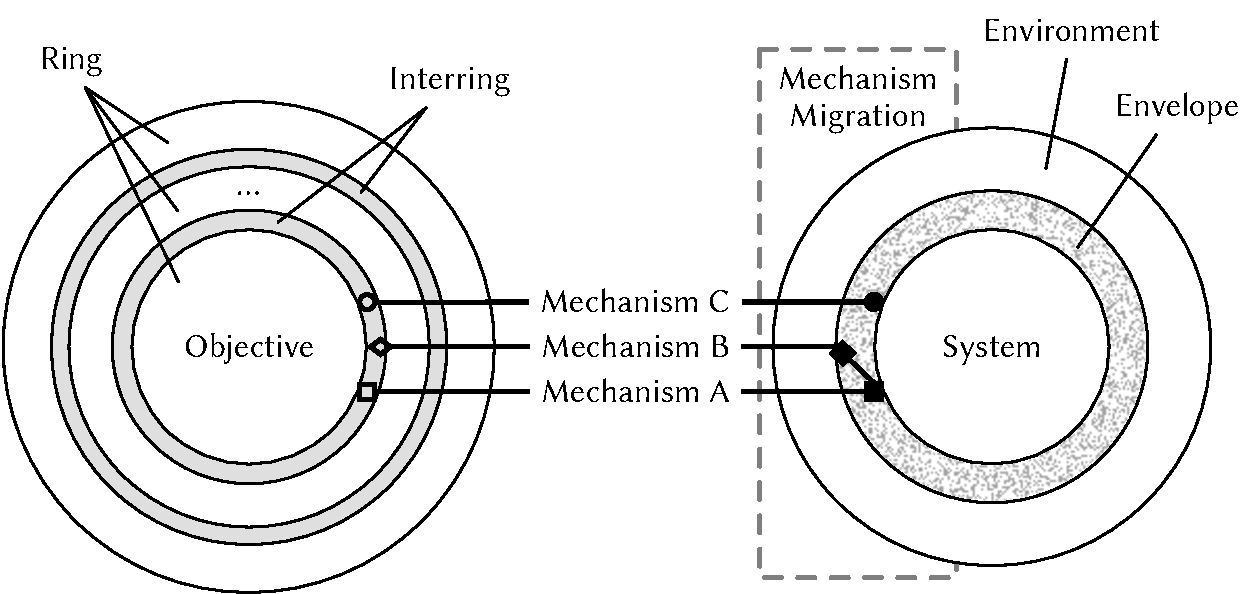
\includegraphics[width=.8\linewidth]{figures/MechanismMigration.pdf}
    \caption{System, Environment and Interceptor Model}
    \label{fig:bigpicture}
\end{figure}


\subsubsection{System and Environment}
At the core of the consideration lies a system that is intended to achieve a specific task.
The system cannot be changed because it contains proprietary components or depends on other external factors, such as high coordination costs for changes due to long standardization or technical hurdles.
In the NAT example above, the system is the host that wants to communicate with hosts in other networks.

Every system is surrounded by an environment that provides functionality to be used by the system.
The system has a dependency relationship with the environment, as the system is dependent on the functions provided.
This is necessary so that the system can fulfill its actual task.
For example, the host in the NAT example needs the routing functionality of the gateway to enable communication with hosts in other networks.

\subsubsection{Mechanism}
By a mechanism, we mean the implementation of a functional unit of the environment that is used by the system to achieve its task~\cite{frommgen2016mechanism}.
% By a mechanism, we refer to ''a confined conceptual element of a (networked) system that is bound to a realization as cooperating functional units''~\cite{frommgen2016mechanism}.
Mechanisms are used by a system via its corresponding interface. 
Mechanisms are located at various points of hardware/software systems, for example:
%
\begin{itemize}
 \item Complete protocols: TCP, UDP, RTP, overlays, etc.
 \item Specific parts of protocols: congestion control, fragmentation, load balancing, replication, etc.
 \item Network concepts: infrastructure-based, ad-hoc, partially meshed, delay tolerant (DTN), etc.
 \item Network technologies: Ethernet, LTE, IEEE 802.11, Bluetooth, etc.
 \item Security mechanisms: encryption, integrity protection, authentication, etc.
 \item System components: positioning (via WLAN, GSM or GPS), sensors, etc.
 \item Operating System APIs: Sockets, Pipes, etc.
 \item System Bus Interfaces: I$^2$C, PCI Express, etc.
\end{itemize}
% Vorschlag: Mechanismen und deren Interfaces aufzählen, statt nur die Interfaces.
%
In the above NAT example, the mechanism provided by the environment that the systems uses is IP routing.


\subsubsection{Unobtrusive Interceptor}
In the field of software engineering, the ``Interceptor architectural pattern allows services to be added transparently to a framework and triggered automatically when certain events occur''~\cite{schmidt2013pattern}.
In this programming pattern, a framework provides interfaces so that programs using the framework can transparently intervene in the flow of data at specific events.
While the goal of our interceptor is basically the same, to transparently intervene in the data flow and thus enable new functionalities, the perspective is reversed.
An interceptor in our definition is part of the environment and provides mechanisms to the system via known interfaces. 
In contrast to the interceptor pattern of software engineering, the interceptor is used by the system but configured by the environment in a way that makes its mandatory.
In order for the system to use the new mechanism, the interceptor is inserted between the system and the mechanism and changes the data flow.
The used mechanism can also be introduced into the environment as part of the interceptor and does not have to exist a priori.
In the above NAT example, the newly added mechanism is IP masquerading as part of the NAT.
The NAT component intervenes with the IP data flow in a way that translates the internal, private IP addresses and TCP/UDP ports with the public IP address and vice-versa.

In order to not influence or even disturb the actual task of the system, the mechanism must be unobtrusively replaced by the provided mechanism of the interceptor.
The system must not notice the change of the mechanism, on the contrary the used interfaces must pretend that the original mechanism is still in place.
Furthermore, an interceptor must be unobtrusive so that the system can continue to fulfill the functionality and not provide error cases for the termination.
